
\subsection{Motorik der Augen} \index{Motorik! Augen}
Die Augenbewegung lässt sich in drei Rotationsachsen einteilen; horizontal, vertikal und rollend (Torsion). Die horizontale Bewegung weg von der Nase wird dabei als Abduktion bezeichnet. Adduktion wird die horizontale Bewegung zur Nase hin genannt. Die vertikale Bewegung des Auges wird entweder durch eine Senkung nach unten oder durch eine Hebung des Augapfels nach oben beschrieben. Zu den Torsionsbewegungen zählen die Innenrollung und die Außenrollung des Auges. Bei einer Innenrollung wird die Spitze der Hornhaut hin zur Nase bewegt, bei einer Außenrollung erfolgt diese Bewegung weg von der Nase in Richtung der Schläfe. Im Normalfall sind die Bewegungen der Augen konjugiert. Dies bedeutet, dass sie immer in dieselbe Richtung erfolgen. Die einzige Ausnahme dabei bildet die Vergenz \textsuperscript{\cite[Kap.~39]{kandel2013principles}}. \\
Das Auge wird durch sechs äußere Augenmuskeln bewegt, welche sich in drei Agonisten-Antagonisten Paare einteilen lassen. Der Musculus rectus medialis und der Musculus rectus lateralis sorgen für eine Horizontalbewegung, wobei der M. rectus medialis die Adduktion und der M. rectus lateralis die Abduktion durchführen. Die restlichen vier Muskeln sind gemeinsam für die vertikalen und rollenden Bewegungen zuständig. Der Musculus rectus superior hebt zusammen mit dem Musculus obliquus inferior das Auge an. Für das Senken sind der Musculus rectus inferior und der Musculus obliquus superior zuständig. Die Innendrehung wird durch die Zusammenarbeit des M. rectus superior und des M. obliquus superior erzeugt, eine Drehung nach Außen durch den M. rectus inferior und M. obliquus inferior \textsuperscript{\cite[Kap.~39]{kandel2013principles}}. \\  
Diese äußere Augenmuskulatur wird durch drei Hirnnerven gesteuert, die aus bestimmten Kerngebieten des Hirnstamms hervorgehen. Der M. rectus lateralis wird durch den VI. Hirnnerv, den Nervus abducens innerviert. Durch den IV. Hirnnerven Nervus trochleraris wird der M. obliquus superior kontrolliert. Die restliche äußere Augenmuskulatur, M. rectus medialis, inferior und superior, sowie M. obliquus inferior, wird komplett durch den III. Hirnnerven Nervus oculomotorius gesteuert \textsuperscript{\cite[Kap.~39]{kandel2013principles}}. Diese Hirnnerven und ihre Kerne werden im Folgenden beschrieben.   

\subsubsection*{III. Hirnnerv: Nervus oculomotorius} \index{Hirnnerven! 03. N. oculomotorius}
Der \textbf{Nervus oculomotorius} besteht zum einen aus somatomotorischen Fasern, die wie oben beschrieben, den Großteil der äußeren Augenmuskulatur innervieren. Zum anderen verlaufen innerhalb des Nervs aber auch viszeromotorische Fasern. Diese steuern über parasympathische Impulse den Musculus sphincter pupillae, der zu einer Verengung der Pupille führt und die Ziliarmuskulatur, die während dem Fokussieren die Krümmung der Linse anpassen \textsuperscript{\cite[Kap.~39]{kandel2013principles}}. Diese Efferenzen stammen dementsprechend auch aus zwei unterschiedlichen Kergebieten, dem \textit{Nucleus nervi oculomotorii}  \index{Nucleus! nervi oculomotorii} und dem \textit{Nucleus accessorius nervi oculomotorii} \index{Nucleus! accessorius nervi oculomotorii} \textsuperscript{\cite[Kap.~5]{trepel2011neuroanatomie}}. \\  
Der Ncl. n. oculomotorii ist im Tegmentum des Mittelhirns, auf Höhe der Colliculi superiories, paramedian kurz vor dem Aquädukt lokalisiert. Die Efferenzen dieses Kerngebiets sind somatomotorisch und für die Innervation von vier der sechs äußeren Augenmuskeln (s.o.) zuständig. Zusätzlich steuert diese Kernregion über den N. oculomotorius den Musculus levator palpebrae superiores, besser bekannt als oberer Lidheber. Im Kontrast dazu wird der Lidschließer über den N. facialis innerviert. Jeder Muskel, der durch den Ncl. n. oculomotorii versorgt wird, nimmt innerhalb des Kerns einen eigenen Bereich ein. Der obere Lidheber beider Augen wird dabei allerdings nur von einem Bereich versorgt. Dieser liegt mittig zwischen dem linken und rechten Ncl. n. oculomotorii. Alle anderen Untergruppen sind paarig angeordnet \textsuperscript{\cite[Kap.~5]{trepel2011neuroanatomie}}. \\
Das Kerngebiet des Ncl. accessorius n. oculomotorii wird auch als \textbf{Edinger-Westphal-Kern} bezeichnet und grenzt mediodorsal an den Ncl. n. oculomotorii an. Über seine parasympatischen Efferenzen innerviert er den Großteil der inneren Augenmuskulatur. Dazu zählt der M. ciliaris, der Einfluss auf die Krümmung der Linse nimmt und der M. sphincter pupillae, welcher für eine Verengung der Pupille sorgt \textsuperscript{\cite[Kap.~5]{trepel2011neuroanatomie}}. \\          
Der Musculus dilatator pupillae fungiert als Antagonist des M. sphincter pupillae und führt dementsprechend zu einer Erweiterung der Pupille. Dieser innere Augenmuskel wird allerdings nicht über den N. oculomotorius gesteuert, sondern steht unter sympathischer Innervation, deren Ursprung im intermediolateralen Bereich des oberen Thorakalsegement der Wirbelsäule liegt \textsuperscript{\cite[Kap.~39]{kandel2013principles}}.

\subsubsection*{IV. Hirnnerv: Nervus trochlearis} \index{Hirnnerven! 04. N. trochlearis}
Innerhalb des \textbf{Nervus trochlearis} verlaufen nur rein somatomotorische Fasern. Diese haben ihren Ursprung im \textit{Nucleus nervi trochlearis} \index{Nucleus! nervi trochlearis} (Abb.~\ref{fig:nucleus_trochlearis}). Dieses Kerngebiet ist im Tegmentum des Mittelhirns auf Höhe der Colliculi inferiores unterhalb des Kernkomplexes des N. oculomotorius lokalisiert \textsuperscript{\cite[Kap.~5]{trepel2011neuroanatomie}}. Die efferenten Fasern verlaufen dorsal um das zentrale Hölengrau herum und kreuzen sofort auf die Gegenseite. Anschließend verlässt er als einziger Hirnnerv dorsal den Hirnnstamm. Von dort verläuft er um die Pedunculus cerebri, um auf die ventrale Seite des Gehirns zu gelangen. Über die Fissura orbitalis superior tritt der N. trochlearis in die Augenhöhle ein, um dort einen Muskel, den M. obliquus superior, zu innervieren \textsuperscript{\cite[Kap.~10]{crossman2014neuroanatomy}}.   

\begin{figure}[H]
    \centering
    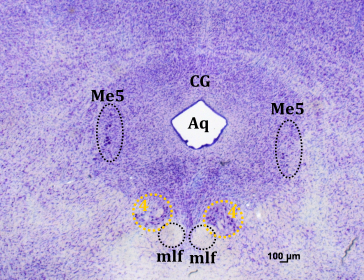
\includegraphics[width=0.7\textwidth]{pictures/Bilder_Laura/nucleus_trochlearis_N14_3M_25x.png}
    \caption[Nucleus nervi trochlearis]{\textbf{Nucleus nervi trochlearis.} Der Nucleus nervi trochlearis (4) ist im Tegmentum des Mittelhirns medial unterhalb des Aquädukts (Aq) zu sehen. Das Aquädukt wird vom zentralen Höhlengrau (CG) umgegeben. Seitlich ist der  Nucleus mesencephalicus nervi trigemini (Me5) zu erkennen. Unterhalb des Ncl. n. trochlearis zieht die Fasciculus longitudinalis medialis (mlf) entlang. Nissl-Färbung (N14-3).}
    \label{fig:nucleus_trochlearis}
\end{figure}

\subsubsection*{VI. Hirnnerv: Nervus abducens} \index{Hirnnerven! 06. N. abducens}
Auch der VI. Hirnnerv, \textbf{Nervus abducens}, besteht aus rein somatomotorischen Fasern, die alle aus einem Kerngebiet, dem \textit{Nucleus nervi abducentis} \index{Nucleus! nervi abducentis}, stammen. Dieser liegt paramedian unterhalb des vierten Ventrikels im caudalen Bereich des Pons. Von dort verlaufen die Fasern ventral durch den Pons und verlassen den Hirnstamm ebenfalls ventral zwischen dem Pons und der Pyramide der Medulla. Der N. abducentis tritt über die Fissura orbitalis superior in die Augenhöhle ein und kontrolliert dort den M. rectus lateralis, welcher für die Abduktion des Auges zuständig ist \textsuperscript{\cite[Kap.~10]{crossman2014neuroanatomy}}. \\    
\\ \noindent Damit die Bewegung des Augapfels perfekt koordiniert werden kann, gibt es internukleare Verbindungen zwischen den drei Kerngebieten, die für die Augenbewegung zuständig sind.    
Eine essentielle reziproke Verbindung besteht dabei zwischen dem Ncl. n. abducentis und dem Ncl. n. oculomotorii. Die Hälfte aller Neurone des Ncl. n. abducentis sind mit dem Subnucleus des M. rectus medialis im Okulomotoriuskern der Gegenseite verbunden. Dadurch lassen sich die Bewegungen des M. rectus medialis und lateralis beider Augen miteinander verknüpfen. Dies hat zur Folge, dass bei der Abduktion des einen Auges das andere adduziert wird und somit die Blickrichtung beider Augen immer übereinstimmt \textsuperscript{\cite[Kap.~6]{trepel2011neuroanatomie}}. 

\subsubsection*{Die Erzeugung vertikaler und horizontaler Augenbewegungen}
Den okulomotorischen Kernen sind höhere, sogenannte \textbf{präokulomotorische Zentren}, vorgeschaltet. Diese Blickzentren sind für die Entstehung der horizontalen und vertikalen Augenbewegungen zuständig \textsuperscript{\cite[Kap.~6]{trepel2011neuroanatomie}}.   
Das Signal für die horizontalen Sakkaden entsteht in der \textbf{paramedianen pontinen Formatio reticularis} (\textbf{PPRF}). Diese Kerngruppe der Formatio reticularis projiziert in den Ncl. n. abducens und initiiert damit horizontale Augenbewegungen zur ipsilateralen Seite \textsuperscript{\cite[Kap.~39]{kandel2013principles}}. Für die Erzeugung der vertikalen Augenbewegungen ist die \textbf{rostrale mesenzephale Formatio reticularis} zuständig. Die Neurone, welche die Signale erzeugen, liegen dabei im rostralen Ncl. interstitialis fasciculi longitudinalis medialis und auch teilweise innerhalb des Ncl. interstitialis Cajal. Ausgehend aus diesen Kerngebieten verlaufen die Axone über die Commissura posterior zum contralateralen Ncl. n. oculomotorius. Von dort wird dann anschließend eine vertikale Augenbewegung generiert
\textsuperscript{\cite[Kap.~6]{trepel2011neuroanatomie}}. \\      
\\ \noindent Die Schaltkreise innerhalb des Mesencephalons und des Pons sind nur für die Erzeugung der motorischen Signale zum Hervorrufen der Sakkaden zuständig. Handelt es sich allerdings um willkürlich durchgeführte Augenbewegungen, sind den präokulomotorischen Kernen noch weitere \textbf{übergeordnete Blickzentren} vorausgeschaltet. Die ultimative Entscheidung eine Sakkade durchzuführen wird im Cortex getroffen. Dazwischen nehmen die Colliculi superiores \index{Colliculus! superior} eine essentielle Funktion ein, um visuelle und motorische Information zu okulomotorischen Signalen zu integrieren und an den Hirnstamm zu senden. Die Colliculi superiores werden dabei von zwei Regionen der Großhirnrinde kontrolliert, vom frontalen Augenfeld \index{frontales Augenfeld} und dem lateralen intraparietalen Bereich des hinteren Parietallappens. Beide Cortexareale tragen zu der Generierung von Sakkaden maßgeblich bei, wobei dem frontalen Augenfeld eine größere Rolle zugesprochen wird \textsuperscript{\cite[Kap.~39]{kandel2013principles}}.             